\documentclass[12pt]{article}\usepackage[]{graphicx}\usepackage[]{color}
%% maxwidth is the original width if it is less than linewidth
%% otherwise use linewidth (to make sure the graphics do not exceed the margin)
\makeatletter
\def\maxwidth{ %
  \ifdim\Gin@nat@width>\linewidth
    \linewidth
  \else
    \Gin@nat@width
  \fi
}
\makeatother

\definecolor{fgcolor}{rgb}{0.345, 0.345, 0.345}
\newcommand{\hlnum}[1]{\textcolor[rgb]{0.686,0.059,0.569}{#1}}%
\newcommand{\hlstr}[1]{\textcolor[rgb]{0.192,0.494,0.8}{#1}}%
\newcommand{\hlcom}[1]{\textcolor[rgb]{0.678,0.584,0.686}{\textit{#1}}}%
\newcommand{\hlopt}[1]{\textcolor[rgb]{0,0,0}{#1}}%
\newcommand{\hlstd}[1]{\textcolor[rgb]{0.345,0.345,0.345}{#1}}%
\newcommand{\hlkwa}[1]{\textcolor[rgb]{0.161,0.373,0.58}{\textbf{#1}}}%
\newcommand{\hlkwb}[1]{\textcolor[rgb]{0.69,0.353,0.396}{#1}}%
\newcommand{\hlkwc}[1]{\textcolor[rgb]{0.333,0.667,0.333}{#1}}%
\newcommand{\hlkwd}[1]{\textcolor[rgb]{0.737,0.353,0.396}{\textbf{#1}}}%

\usepackage{framed}
\makeatletter
\newenvironment{kframe}{%
 \def\at@end@of@kframe{}%
 \ifinner\ifhmode%
  \def\at@end@of@kframe{\end{minipage}}%
  \begin{minipage}{\columnwidth}%
 \fi\fi%
 \def\FrameCommand##1{\hskip\@totalleftmargin \hskip-\fboxsep
 \colorbox{shadecolor}{##1}\hskip-\fboxsep
     % There is no \\@totalrightmargin, so:
     \hskip-\linewidth \hskip-\@totalleftmargin \hskip\columnwidth}%
 \MakeFramed {\advance\hsize-\width
   \@totalleftmargin\z@ \linewidth\hsize
   \@setminipage}}%
 {\par\unskip\endMakeFramed%
 \at@end@of@kframe}
\makeatother

\definecolor{shadecolor}{rgb}{.97, .97, .97}
\definecolor{messagecolor}{rgb}{0, 0, 0}
\definecolor{warningcolor}{rgb}{1, 0, 1}
\definecolor{errorcolor}{rgb}{1, 0, 0}
\newenvironment{knitrout}{}{} % an empty environment to be redefined in TeX

\usepackage{alltt}  
\usepackage{amsfonts, amsmath, amsthm, amssymb, enumitem, verbatim, graphicx}
\setlength{\parindent}{0pt}
\setlength{\parskip}{1ex plus 0.5ex minus 0.2ex}
\usepackage [margin=1in, paperwidth=8.5in, paperheight=11in]{geometry}

\newcommand{\bfbeta}{\mbox{\boldmath $\beta$}}
\newcommand{\bfX}{\mbox{\boldmath $X$}}
\newcommand{\bfV}{\mbox{\boldmath $V$}}
\newcommand{\bfI}{\mbox{\boldmath $I$}}
\newcommand{\bfy}{\mbox{\boldmath $y$}}
\newcommand{\bfeps}{\mbox{\boldmath $\epsilon$}}
\IfFileExists{upquote.sty}{\usepackage{upquote}}{}
\begin{document}


{ \flushright Jordan Schupbach \\
STAT 532\\
September 2, 2015 \\}
Homework \# 1\\

\begin{enumerate}
\item Since we have $X ~HypG(12, \theta, 5)$, we can use the function \texttt{dhyper()} to obtain \newline $Pr(X=x| \theta)$ for specific values of $x$ and $\theta$.

\item To draw one gold ball for a specific value of $\theta$, have the following function
\begin{verbatim}
hyp_theta <- function(theta, x = 1){
  dhyper(x, theta, 12 - theta, 5)
}
\end{verbatim}
\item To create a 2-way table of $Pr(X=x | \theta)$ for $X=0, \dots, 5$ and $\theta = 0, \dots, 12$ using the function above, we can use the \texttt{mapply()} function by the following.

\begin{verbatim}
matrix(mapply(hyp_theta, theta = c(rep(0, 6), rep(1,6), rep(2,6), rep(3,6), 
       rep(4,6), rep(5, 6),rep(6, 6), rep(7,6), rep(8,6), rep(9,6), rep(10,6), 
       rep(11, 6), rep(12,6)), x = c(rep(0:5, 13))), 13, 6, byrow = T)
\end{verbatim}

Another option in building this table is to use a \texttt{for} loop as in the code below:

\begin{verbatim}
tab1 <- matrix(rep(NA, 6*13), 13, 6)
for(i in 0:5){
  tab1[, i+1] <- dhyper(i, 0:12, 12:0,5)
}
\end{verbatim}

\newpage 
Code is provided in the appendix to clean this up into the table given below.

% latex table generated in R 3.2.1 by xtable 1.7-4 package
% Wed Sep  2 09:52:40 2015
\begin{table}[ht]
\centering
\begin{tabular}{rrrrrrrl}
  \hline
 & 0 & 1 & 2 & 3 & 4 & 5 & Row Sums \\ 
  \hline
0 & 1.000 & 0.000 & 0.000 & 0.000 & 0.000 & 0.000 & 1 \\ 
  1 & 0.583 & 0.417 & 0.000 & 0.000 & 0.000 & 0.000 & 1 \\ 
  2 & 0.318 & 0.530 & 0.152 & 0.000 & 0.000 & 0.000 & 1 \\ 
  3 & 0.159 & 0.477 & 0.318 & 0.045 & 0.000 & 0.000 & 1 \\ 
  4 & 0.071 & 0.354 & 0.424 & 0.141 & 0.010 & 0.000 & 1 \\ 
  5 & 0.027 & 0.221 & 0.442 & 0.265 & 0.044 & 0.001 & 1 \\ 
  6 & 0.008 & 0.114 & 0.379 & 0.379 & 0.114 & 0.008 & 1 \\ 
  7 & 0.001 & 0.044 & 0.265 & 0.442 & 0.221 & 0.027 & 1 \\ 
  8 & 0.000 & 0.010 & 0.141 & 0.424 & 0.354 & 0.071 & 1 \\ 
  9 & 0.000 & 0.000 & 0.045 & 0.318 & 0.477 & 0.159 & 1 \\ 
  10 & 0.000 & 0.000 & 0.000 & 0.152 & 0.530 & 0.318 & 1 \\ 
  11 & 0.000 & 0.000 & 0.000 & 0.000 & 0.417 & 0.583 & 1 \\ 
  12 & 0.000 & 0.000 & 0.000 & 0.000 & 0.000 & 1.000 & 1 \\ 
  Col Sums & 2.167 & 2.167 & 2.167 & 2.167 & 2.167 & 2.167 &  \\ 
   \hline
\end{tabular}
\end{table}


The columns are for specific values of $X$ and the rows are for specific values of $\theta$.

\item (combined in 3 and 5)
\item In the table above, notice that the rows sum to 1. This is because $Pr(X = x | \theta)$ is a probability function across its entire domain. However, the columns do not sum to 1. This shows that the columns of the table do not represent a probability function. Rather, it is simply a function of $\theta$ given specific values of $\theta$. For this reason, we do not use $Pr( \theta | X)$ for our notation, but rather we use $L(\theta | X)$. We use $L$ for  ''likelihood'' to describe values of $\theta$ given an outcome $X$.

\item To find our ''Maximum Likelihood Estimator'', we find the max of $L(\theta | X)$. In this context, a discrete one, we simply take the largest of the values in each column. For instance, if we observe 3 gold balls in our sample of 5, our MLE for $\theta$ is $\hat{\theta} = 7$ since the $.442$ is the largest number in the column associated with $X = 3$.

\item An {\bf estimator} is a process that yields an {\bf estimate} given the data. Thus, when we talk about an {\bf estimator}, we are talking about the process that yields different {\bf estimates} given the data. Whereas, when we say {\bf estimate}, we have observed the data and can now calculate the {\bf estimate} from our {\bf estimator}.

\item The Maximum Likelihood {\bf Estimator} for this problem can take on the values $ \{0, 2, 5, 7, 10, 12 \}$. We can obtain these values by finding the largest value in the table above for each column, where the row for the maximum value gives the associated Maximum Likelihood {\bf Estimate} given the value of $X$, the observed data. 
\newpage

\item The table below gives the maximum likelihood estimates associated with the different possible values of $X$. For each observed $X$, we have an associated value of $\hat{\theta}$ \\

\begin{center}
\begin{tabular}{|c|c|}
\hline
$X$ & $\hat{\theta}$ \\
\hline
0 & 0\\
1 & 2\\
2 & 5\\
3 & 7\\
4 & 10\\
5 & 12\\
\hline
\end{tabular}
\end{center}

\item 
\begin{enumerate}[label=(\alph*)]
\item If we observe 1 gold ball, we have $\hat{\theta} = 2$. That is, if in our experiment, one of the five balls drawn is gold, our estimate of the true number of gold balls in the bucket based on the maximum likelihood estimator is 2.
\item
Given that we observe 1 gold ball, we have the following plot of the likelihood function. 

\begin{knitrout}
\definecolor{shadecolor}{rgb}{0.969, 0.969, 0.969}\color{fgcolor}

{\centering 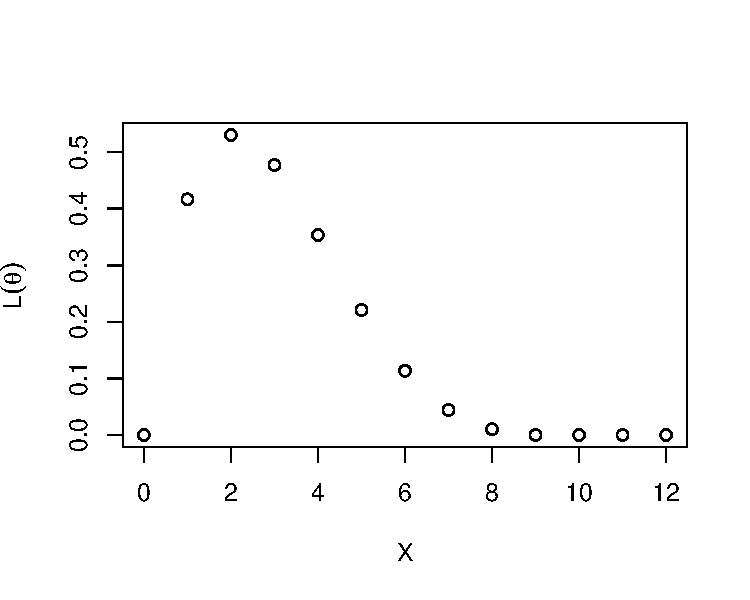
\includegraphics[width=\maxwidth]{figure/plot9a-1} 

}



\end{knitrout}

We do not plot a histogram here as that would suggest that values between the integers from 0 to 12 are meaningful. However, in the context of this problem, the number of balls in the bucket can only take on integer values (from 0 to 12).
\newpage
\item Below, we plot the ''normalized'' likelihood function.

\begin{knitrout}
\definecolor{shadecolor}{rgb}{0.969, 0.969, 0.969}\color{fgcolor}

{\centering 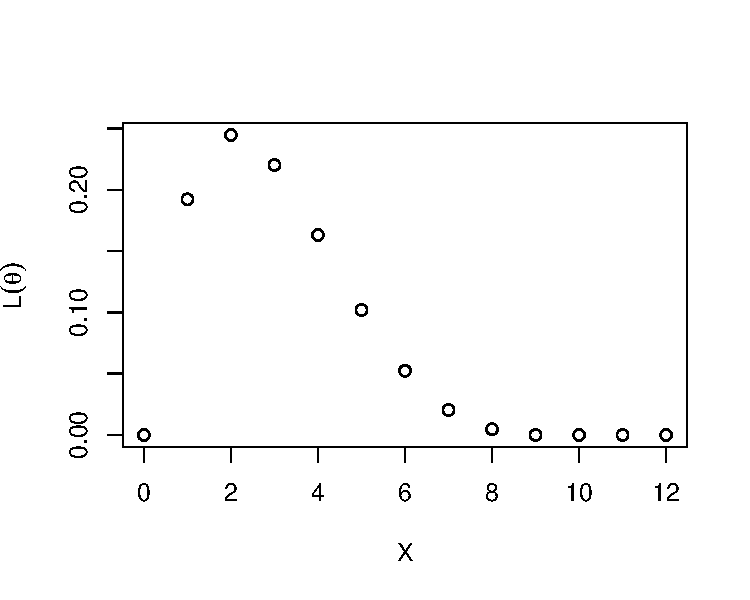
\includegraphics[width=\maxwidth]{figure/plot9b-1} 

}



\end{knitrout}

They are ''normalized'' in that now $L(\theta|X=1)$ represents a probability function in that summing over all possible values of $\theta$ gives 1 rather than $2.1\overline{66}$ as in before. 
\end{enumerate}

\item

\begin{enumerate}[label=(\alph*)]
\item 
When we use the function \texttt{lm()}, R is finding the Best Linear Unbiased Estimators (BLUE's) for $\bfbeta$ by calculating $\hat{\bfbeta} = (\bfX^T \bfX)^{-1} \bfX^T \bfy$ where we the model $\bfy = \bfX \bfbeta + \bfeps$  with $\bfeps \overset{iid}{\sim} (0, \sigma^2 \bfI)$. Whereas, when we use the function \texttt{glm()}, R is using an iteratively reweighted (IWLS) algorithm to calculate the Maximum Likelihood Estimates for $\bfbeta$ (and $\sigma^2$). Here we still have the model $\bfy = \bfX \bfbeta + \bfeps$  with $\bfeps \overset{iid}{\sim} (0, \sigma^2 \bfI)$. Now, we no longer have BLUE's, however the MLE's are asymptotically efficient (as sample size goes to infinity). 

\item Confidence intervals for each are obtained in quite a different manner. Consider the \texttt{confint()} function in R which has methods for both \texttt{lm()} and \texttt{glm()}. For \texttt{lm()}, R simply calculates the confidence interval as $\hat{\beta} \pm t_{n-k, \alpha} \times SE(\hat{\beta})$ where k is the number of parameters in the model. However, in the method for \texttt{glm()}, R calculates confidence intervals through profiling the associated likelihoods. In the details section for this function (from the MASS package), the authors describe the method for making this calculation. They write, ''These confint methods call the appropriate profile method, then find the confidence intervals by interpolation in the profile traces.''

\end{enumerate}
\item We have
$$P(\theta | x) = \dfrac{P(x|\theta) P(\theta) }{P(x)} $$

In the context of the bucket problem, we have
\begin{align*}
P(\theta | x) &= \dfrac{P(x|\theta) P(\theta) }{P(x)}\\
&= \dfrac{f(x|\theta) g(\theta) }{h(x)}\\
&= \dfrac{ \dfrac{{ \theta \choose x} {12 - \theta \choose 5 - x}}{{12 \choose 5}} g(\theta) }{h(x)}\\
\end{align*}
However, we need to know (or assume) $g(\theta)$, our prior distribution, to finish the calculation.

\item As stated in the previous problem, to obtain the posterior distribution for the bucket problem, we must first assume a prior distribution. We shall, as before, call this $g(\theta)$. Thus, we can use the likelihood function to calculate the posterior distribution as follows:

\begin{align*}
P(\theta | x) &= \dfrac{P(x|\theta) P(\theta) }{P(x)}\\
&= \dfrac{f(x|\theta) g(\theta) }{h(x)}\\
&= \dfrac{L(\theta|X) g(\theta) }{h(x)}\\
&= \dfrac{L(\theta|X) g(\theta) }{\sum_{i=0}^{12} L(\theta_i|X) g(\theta_i)}\\
\end{align*}
\newpage
\item 
\begin{enumerate}[label=(\alph*)]
\item For this prior, we have
\begin{table}[ht]
\centering
\begin{tabular}{ccccc}
  \hline
$\theta$ & $g(\theta)$ & $L(\theta | X=1)$  & $L(\theta | X=1) * g(\theta)$ & $f(\theta | X=1)$ \\ 
  \hline
0 & 0.0000 & 0.0000 & 0.0000 & 0.0000 \\ 
1 & 0.0000 & 0.4167 & 0.0000 & 0.0000 \\ 
2 & 0.0278 & 0.5303 & 0.0147 & 0.1230 \\ 
3 & 0.0556 & 0.4773 & 0.0265 & 0.2213 \\ 
4 & 0.0833 & 0.3535 & 0.0295 & 0.2459 \\ 
5 & 0.1111 & 0.2210 & 0.0246 & 0.2049 \\ 
6 & 0.1389 & 0.1136 & 0.0158 & 0.1317 \\ 
7 & 0.1667 & 0.0442 & 0.0074 & 0.0615 \\ 
8 & 0.1389 & 0.0101 & 0.0014 & 0.0117 \\ 
9 & 0.1111 & 0.0000 & 0.0000 & 0.0000 \\ 
10 & 0.0833 & 0.0000 & 0.0000 & 0.0000 \\ 
11 & 0.0556 & 0.0000 & 0.0000 & 0.0000 \\ 
12 & 0.0278 & 0.0000 & 0.0000 & 0.0000 \\ 
   \hline
\end{tabular}
\end{table}

\item For this prior, we have

\begin{table}[ht]
\centering
\begin{tabular}{ccccc}
  \hline
$\theta$ & $g(\theta)$ & $L(\theta | X=1)$  & $L(\theta | X=1) * g(\theta)$ & $f(\theta | X=1)$ \\ 
  \hline
0 & 0.0000 & 0.0000 & 0.0000 & 0.0000 \\ 
1 & 0.1667 & 0.4167 & 0.0694 & 0.1973 \\ 
2 & 0.1667 & 0.5303 & 0.0884 & 0.2510 \\ 
3 & 0.1667 & 0.4773 & 0.0795 & 0.2259 \\ 
4 & 0.1667 & 0.3535 & 0.0589 & 0.1674 \\ 
5 & 0.1667 & 0.2210 & 0.0368 & 0.1046 \\ 
6 & 0.1667 & 0.1136 & 0.0189 & 0.0538 \\ 
7 & 0.0000 & 0.0442 & 0.0000 & 0.0000 \\ 
8 & 0.0000 & 0.0101 & 0.0000 & 0.0000 \\ 
9 & 0.0000 & 0.0000 & 0.0000 & 0.0000 \\ 
10 & 0.0000 & 0.0000 & 0.0000 & 0.0000 \\ 
11 & 0.0000 & 0.0000 & 0.0000 & 0.0000 \\ 
12 & 0.0000 & 0.0000 & 0.0000 & 0.0000 \\ 
   \hline
\end{tabular}
\end{table}

\newpage
\item For this prior, we have

\begin{table}[ht]
\centering
\begin{tabular}{rrrrrr}
  \hline
$\theta$ & $g(\theta)$ & $L(\theta | X=1)$  & $L(\theta | X=1) * g(\theta)$ & $f(\theta | X=1)$ \\
  \hline
0 & 0.0002 & 0.0000 & 0.0000 & 0.0000 \\ 
1 & 0.0029 & 0.4167 & 0.0012 & 0.0078 \\ 
2 & 0.0161 & 0.5303 & 0.0085 & 0.0547 \\ 
3 & 0.0537 & 0.4773 & 0.0256 & 0.1641 \\ 
4 & 0.1208 & 0.3535 & 0.0427 & 0.2734 \\ 
5 & 0.1934 & 0.2210 & 0.0427 & 0.2734 \\ 
6 & 0.2256 & 0.1136 & 0.0256 & 0.1641 \\ 
7 & 0.1934 & 0.0442 & 0.0085 & 0.0547 \\ 
8 & 0.1208 & 0.0101 & 0.0012 & 0.0078 \\ 
9 & 0.0537 & 0.0000 & 0.0000 & 0.0000 \\ 
10 & 0.0161 & 0.0000 & 0.0000 & 0.0000 \\ 
11 & 0.0029 & 0.0000 & 0.0000 & 0.0000 \\ 
12 & 0.0002 & 0.0000 & 0.0000 & 0.0000 \\ 
   \hline
\end{tabular}
\end{table}
\end{enumerate}

\item We have the following plots of $f(\theta | X=1)$ for the three preceeding situations. 

\begin{knitrout}
\definecolor{shadecolor}{rgb}{0.969, 0.969, 0.969}\color{fgcolor}

{\centering 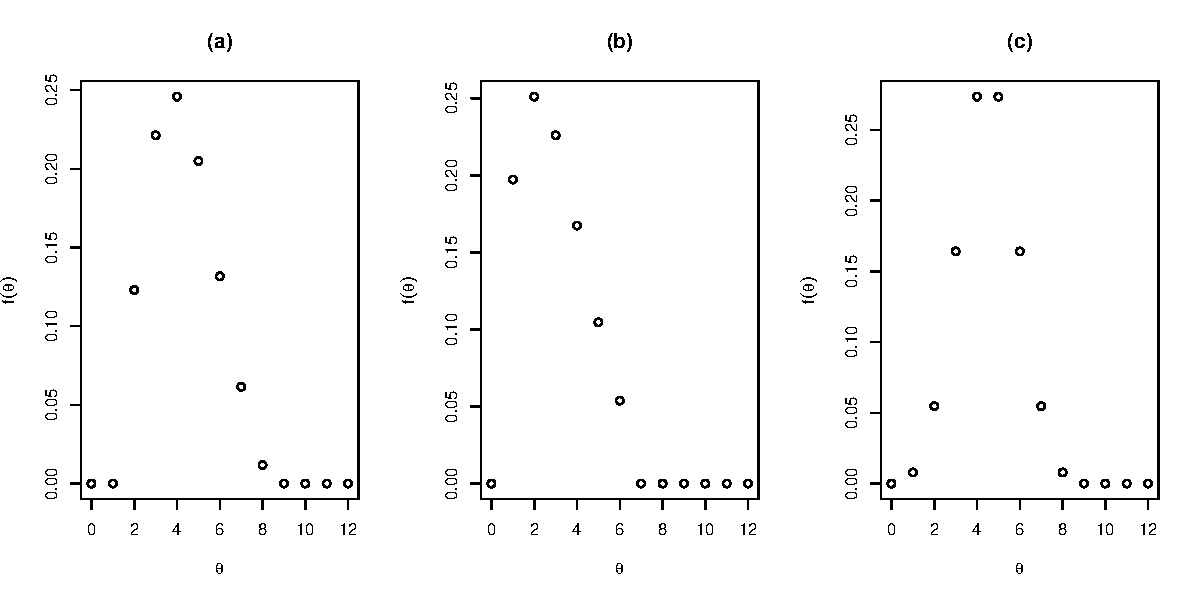
\includegraphics[width=\maxwidth]{figure/plot15-1} 

}



\end{knitrout}

The probabilities shown in the plots make intuitive sense for the three situations given each prior. For (a), we have $f(\theta | X=1) = 0$ for $\theta \in \{ 0, 1, 9, 10, 11, 12\}$ since $g(\theta) = 0$ for $\theta \in \{0, 1, 3 \}$ and $L(\theta | X=1) = 0$ for $\theta \in \{9, 10, 11, 12 \}$. In fact, since all three share the same likelihood, $f(\theta | X=1) = 0$ for $\theta \in \{,  10, 11, 12 \}$ in each case. In (b), we see that $f(\theta | X=1) = 0$ additionally for $\{ 7, 8\}$ since the prior probabilities are zero for each. In (c), the only values for which  $f(\theta | X=1) = 0$ are the ones for which $L(\theta | X=1) = 0$  since all prior probabilities are positive.

\item None of the posterior distributions above match the normalized likelihood function in problem 10 since the process of normalizing the likelihood function is equivalent to picking the non-informative prior. That is, we have $g(\theta) = \dfrac{1}{13} \underset{\{0, 1, \dots, 12 \}}{I(\theta)}$, putting equal probability on each point of the prior. 

\item The situation is complicated in that we have to make some somewhat non-informed decisions about our priors. For instance in (a), since we know the filler has a strong preference for the color blue, we have to decide what exactly that means. Do we think that the probability of the prior for say $\theta =4$ is much higher than for $\theta =8$, or do we think $P(\theta = 8) = 0$? Below, we draw some possible shapes for the prior distributions given the problem descriptions. 
\begin{enumerate}[label=(\alph*)]
\item For a ''strong'' preference for blue, a possible prior distribution we might assume is
\begin{knitrout}
\definecolor{shadecolor}{rgb}{0.969, 0.969, 0.969}\color{fgcolor}

{\centering 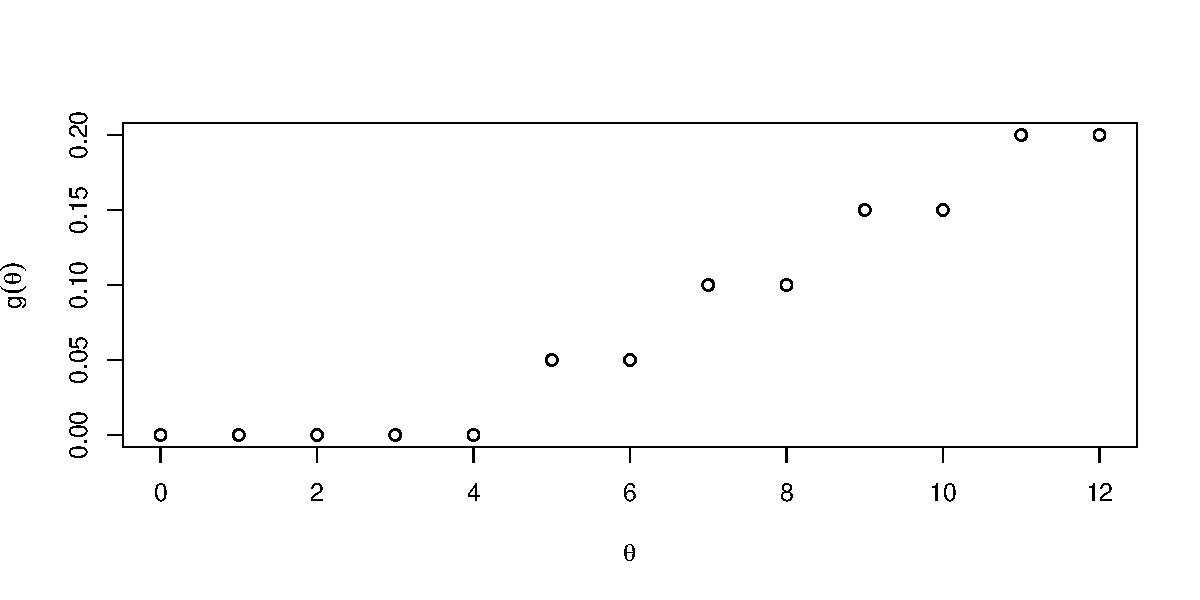
\includegraphics[width=\maxwidth]{figure/plot17a-1} 

}



\end{knitrout}
\item If we think the fillers almost always chose equal composition of gold and blue, we may have a prior that looks like this.

\begin{knitrout}
\definecolor{shadecolor}{rgb}{0.969, 0.969, 0.969}\color{fgcolor}

{\centering 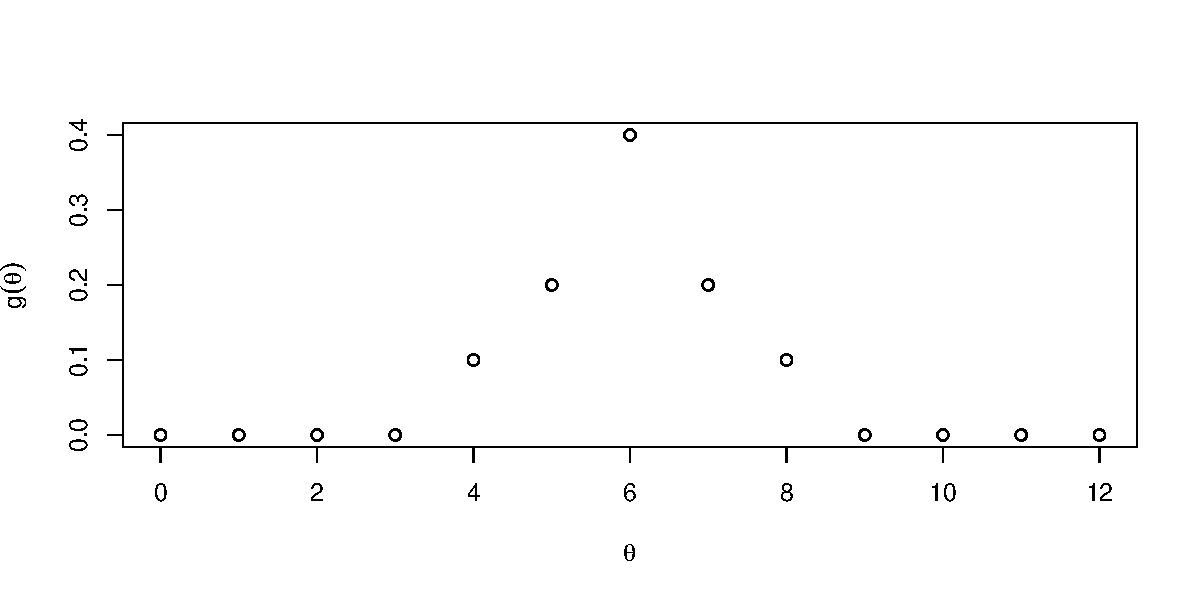
\includegraphics[width=\maxwidth]{figure/plot17b-1} 

}



\end{knitrout}

\item If we notice that all fillers put more of one color than the other, we may assume a prior that looks like this. 

\begin{knitrout}
\definecolor{shadecolor}{rgb}{0.969, 0.969, 0.969}\color{fgcolor}

{\centering 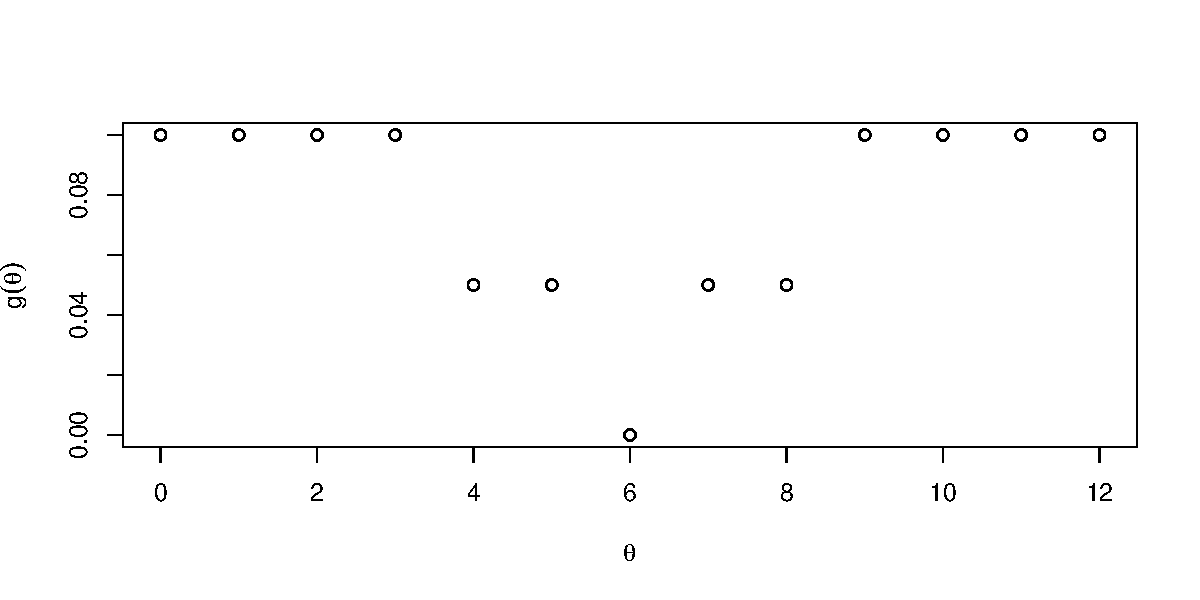
\includegraphics[width=\maxwidth]{figure/plot17c-1} 

}



\end{knitrout}
\item If we have no knowledge about how they might fill the bucket, we may just want to put equal probabilities on each outcome.

\begin{knitrout}
\definecolor{shadecolor}{rgb}{0.969, 0.969, 0.969}\color{fgcolor}

{\centering 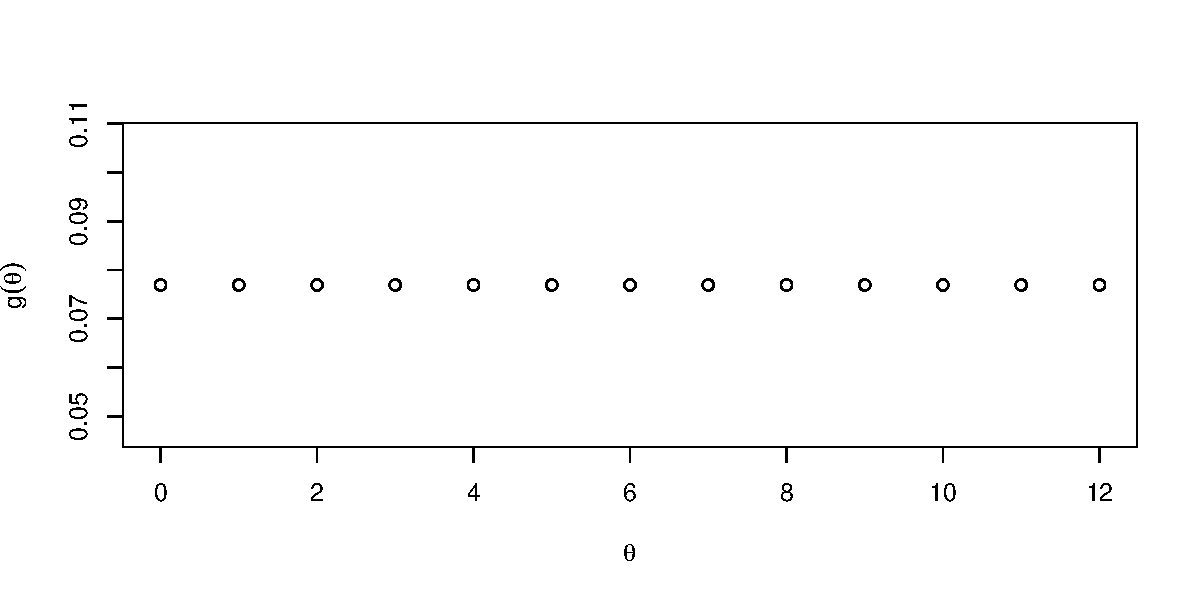
\includegraphics[width=\maxwidth]{figure/plot17d-1} 

}



\end{knitrout}
\end{enumerate}

\end{enumerate}
\newpage
\section*{R-Code}
\begin{verbatim}

## Require Packages
require(xtable)

# Problem 3
tab1 <- matrix(rep(NA, 6*13), 13, 6)
for(i in 0:5){
  tab1[, i+1] <- dhyper(i, 0:12, 12:0,5)
}

tab1 <- cbind(tab1, apply(tab1, 1, sum))
tab1 <- rbind(tab1, apply(tab1, 2, sum))

dimnames(tab1) <- list(c(0:12, "Col Sums"), c(0:5, "Row Sums"))
tab1 <- as.data.frame(tab1)
tab1[14,7] <- ""
xtable(tab1, digits = 3)

# Problem 9
plot(0:12, tab1[1:13,2], xlab = "X", ylab = expression(L(theta)))

#Problem 14
#a
g <- c(0,0,1/36,2/36,3/36,4/36,5/36,6/36,5/36,4/36,3/36,2/36,1/36)
l <- tab1[1:13,2]
gl <- g*l
f <- gl / sum(gl)
tab2 <- cbind(0:12, g, l, gl, f)
xtable(tab2, digits = 4)

#b
g <- c(0,1/6,1/6,1/6,1/6,1/6,1/6,0,0,0,0,0,0)
l <- tab1[1:13,2]
gl <- g*l
f <- gl / sum(gl)
tab3 <- cbind(0:12, g, l, gl, f)
xtable(tab3, digits = 4)

#c
g <- dbinom(0:12, 12, .5)
l <- tab1[1:13,2]
gl <- g*l
f <- gl / sum(gl)
tab4 <- cbind(0:12, g, l, gl, f)
xtable(tab4, digits = 4)

#Problem 17
#a
par(mfrow = c(1,1))
g <- c(0,0,0,0, 0,1/20, 1/20, 1/10, 1/10, 3/20, 3/20, 2/10, 2/10)
plot(0:12, g, xlab = expression(theta), ylab = expression(g(theta)))
#b
g <- c(0,0,0,0, 1/10,1/5, 2/5, 1/5, 1/10, 0, 0, 0, 0)
plot(0:12, g, xlab = expression(theta), ylab = expression(g(theta)))
#c
g <- c(1/10,1/10,1/10,1/10, 1/20,1/20, 0, 1/20, 1/20, 1/10, 1/10, 1/10, 1/10)
plot(0:12, g, xlab = expression(theta), ylab = expression(g(theta)))
#d
g <- rep(1/13, 13)
plot(0:12, g, xlab = expression(theta), ylab = expression(g(theta)))
\end{verbatim}
\end{document})
